\documentclass[11pt]{article}

\usepackage[utf8]{inputenc}

\usepackage{graphicx}
\graphicspath{{assets/}}
\usepackage[francais]{babel}
\usepackage{listings}
\usepackage{float}

%https://mysnippets443.wordpress.com/2015/11/28/latex-insert-javascript-code-with-lstlisting-package/


%Define the listing package
\usepackage{listings} %code highlighter
\usepackage{color} %use color
\definecolor{mygreen}{rgb}{0,0.6,0}
\definecolor{mygray}{rgb}{0.5,0.5,0.5}
\definecolor{mymauve}{rgb}{0.58,0,0.82}
 
%Customize a bit the look
\lstset{ %
backgroundcolor=\color{white}, % choose the background color; you must add \usepackage{color} or \usepackage{xcolor}
basicstyle=\footnotesize, % the size of the fonts that are used for the code
breakatwhitespace=false, % sets if automatic breaks should only happen at whitespace
breaklines=true, % sets automatic line breaking
captionpos=b, % sets the caption-position to bottom
commentstyle=\color{mygreen}, % comment style
deletekeywords={...}, % if you want to delete keywords from the given language
escapeinside={\%*}{*)}, % if you want to add LaTeX within your code
extendedchars=true, % lets you use non-ASCII characters; for 8-bits encodings only, does not work with UTF-8
frame=single, % adds a frame around the code
keepspaces=true, % keeps spaces in text, useful for keeping indentation of code (possibly needs columns=flexible)
keywordstyle=\color{blue}, % keyword style
% language=Octave, % the language of the code
morekeywords={*,...}, % if you want to add more keywords to the set
numbers=left, % where to put the line-numbers; possible values are (none, left, right)
numbersep=5pt, % how far the line-numbers are from the code
numberstyle=\tiny\color{mygray}, % the style that is used for the line-numbers
rulecolor=\color{black}, % if not set, the frame-color may be changed on line-breaks within not-black text (e.g. comments (green here))
showspaces=false, % show spaces everywhere adding particular underscores; it overrides 'showstringspaces'
showstringspaces=false, % underline spaces within strings only
showtabs=false, % show tabs within strings adding particular underscores
stepnumber=1, % the step between two line-numbers. If it's 1, each line will be numbered
stringstyle=\color{mymauve}, % string literal style
tabsize=2, % sets default tabsize to 2 spaces
title=\lstname % show the filename of files included with \lstinputlisting; also try caption instead of title
}
%END of listing package%
 
\definecolor{darkgray}{rgb}{.4,.4,.4}
\definecolor{purple}{rgb}{0.65, 0.12, 0.82}
 
%define Javascript language
\lstdefinelanguage{JavaScript}{
keywords={typeof, new, true, false, catch, function, return, null, catch, switch, var, if, in, while, do, else, case, break},
keywordstyle=\color{blue}\bfseries,
ndkeywords={class, export, boolean, throw, implements, import, this},
ndkeywordstyle=\color{darkgray}\bfseries,
identifierstyle=\color{black},
sensitive=false,
comment=[l]{//},
morecomment=[s]{/*}{*/},
commentstyle=\color{purple}\ttfamily,
stringstyle=\color{red}\ttfamily,
morestring=[b]',
morestring=[b]"
}
 
\lstset{
language=JavaScript,
extendedchars=true,
basicstyle=\footnotesize\ttfamily,
showstringspaces=false,
showspaces=false,
numbers=left,
numberstyle=\footnotesize,
numbersep=9pt,
tabsize=2,
breaklines=true,
showtabs=false,
captionpos=b
}



\begin{document}

\title{Candide 2.0 ou l'optimisme en jeu vidéo }
\author{Nina Ionescu 3mg01 \\ Mentor : Jean-Marc Ledermann \\ Lycée Denis de Rougemont}
\date{}
\pagenumbering{gobble}
\maketitle

\includegraphics{title}
\newpage
\tableofcontents
\newpage
\pagenumbering{arabic}
\section{Introduction}\
\textit {Il y avait en Westphalie...} Et si cet incipit mythique se retrouvait un jour pixelisé, cela donnerait quoi ? C'est ce à quoi j'ai essayé de répondre lors de ce travail de maturité, qui consistait à adapter le premier chapitre dans \textit{Candide} de Voltaire en un jeu vidéo de type RPG (jeu de rôle).
% mettre des screenshots et ue brève explication du jeu plus références à Candide
\begin{figure}[h]

\includegraphics[scale=0.33]{ecranTitre}
\end{figure}
\subsection{Lexique}
Afin d'avoir une meilleure compréhension de ce document, voici un lexique. \\
\begin{itemize}{}{}
\item assets : Désigne l'ensemble des fichiers visuels et auditifs du jeu.
\item frame: Image constituant une partie de l'animation d'un sprite.
\item hp: Abréviation de health points, points de vie.
\item map: Carte.
\item overworld: Monde extérieur en français. Désigne l'ensemble de maps constituant le jeu.
\item pixel art : Style graphique inspiré des jeux rétros où les assets sont dessinés à la main en respectant certains formats.
\item pnj: Abréviation de personnage non-jouable.
\item sprite: Image du jeu en partie transparente capable de déplacement.
\item spritesheet: Image regroupant les frames d'animation d'un sprite.
\item tile : Carreau en français; petite image carrée à texture répétée.
\item tilemap: Carte à carreaux en français. Carte du jeu formée par des tiles.
\item tileset: Ensemble de tiles sous forme de spritesheet.
\item warp: Zone qui une fois pénétrée déclenche un changement de map.
\end{itemize}

\section{Déroulement du jeu PAS FINI}
% personnages , dessiner
Le joueur incarne Candide et peut se promener dans des situations inspirées du livre. Il peut dialoguer avec les pnjs présents dans les décors et faire des combats avec certains d'entre eux. Le joueur arrive dans la cour du château du Baron de Thunder-then-Tronck. 
\begin{figure}[h]
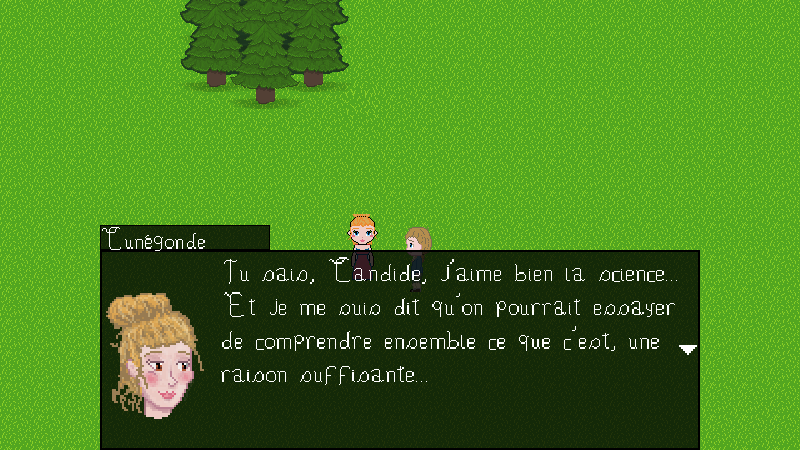
\includegraphics[scale=0.33]{cunegondeScn}
\centering
\end{figure}
sources : \
Phaser.js par Richard Davey \
Phaser-tilemap-plus par Colin Vella \
Bosca Ceoil par Terry Cavanagh \
Pyxel Edit par Danik ( pseudonyme )\


\section{Fonctionement du code}
Ce projet a été réalisé en javascript, avec les additions de ECMAScript6 et de deux librairies conçues pour la réalisation de jeu-vidéo : Phaser.js ainsi que Phaser-tilemap-plus.js . La majorité du code comprend des objets et des classes créés afin de pouvoir les utiliser comme outils de création.
\subsection{Système général}
	Avant toute chose, il a fallu concevoir un système qui permette d'atteindre diverses variables au travers de tous les outils du jeu. C'est pourquoi l'objet "globals" (présent dans globals.js), une variable globale a été créée. Cet objet stocke toutes les variables afin d'y avoir accès facilement sans devoir se soucier des scopes des différentes classes et de leur méthodes.\\\\
	(Pour retenir les diverses actions effectuées par le joueur ainsi que des données importantes telles que son positionnement ou le décor actuellement chargé à l'écran, un autre objet global (présent dans gameRef.js) est utilisé. Il sert de référence pour initialiser le personnage incarné par le joueur dans l'état où ce dernier l'avait laissé.)\\\\ (pas encore sûre, voir le local storage)
 
 Afin d'étendre les possibilités futures de diffusion du projet, une option de traduction a été pensée dans le code de départ. Il s'agit d'un chiffre ( 0 pour le français, 1 pour l'anglais, ... ) stocké dans l'objet mentionné au paragraphe ci-dessus. Grâce à cette variable, la fonction de dialogList.js retourne les textes figurants dans le jeu dans leur bonne version. \\
 \begin{lstlisting}[language=JavaScript]
 function setDialog(langue){
    switch(langue){
        case 0 : 
        globals.dialogs.myChar=["Bonjour"];
    break;
        case 1:
        globals.dialogs.myChar=["Hello"];
		break;
 	}
 }
\end{lstlisting}
\textit{Exemple de la fonction traductrice pour le dialogue d'un personnage quelconque}
\subsection{Gestion des states du jeu}
%qu'est-ce qu'une state, comment ça marche etc...\\\\
Les states, propres à Phaser.js, représentent une section du jeu. Chaque objet state a son lot de fonctions Phaser, à savoir preload, create, update et render. L'utilisation de ces fonctions va être décrite dans les paragraphes ci-dessous.

\subsubsection{Boot et Preload}
%boot fait démarrer le jeu, preload pour les assets etc...
La state "Boot" fait démarrer le jeu. Elle déclenche la state "Preload". Preload est une state qui utilise uniquement la fonction preload, qui sert à associer tous les assets du jeu à un nom et les stocker dans le cache pour pouvoir les utiliser dans le code. Une fois tous les éléments stockés, la state "Menu principal" est enclenchée. Le choix d'utiliser une unique state pour ce travail permet une meilleure organisation au sein du code.
\subsubsection{Menu Principal}
%expliquer la fonction avec les boutons, dans un premier temps elle est avec une sprite sheet pour chaque langue, éventuelle amélioration.\\
La state "menu principal" permet au joueur de lancer le jeu ou d'en modifier la langue. Les boutons qui permettent de faire une action sont des objets Phaser. L'ensemble des boutons est initié dans une seule fonction. Cette fonction dépend de la langue que le joueur a choisi. Chaque bouton a sa propre spritesheet, ce qui pourrait poser problème au niveau de la taille et du temps pour les dessiner si d'autres langues sont ajoutées. Une option serait de générer dans le code, les textes dans les boutons à la place de les dessiner à la main.
\begin{figure}[h]
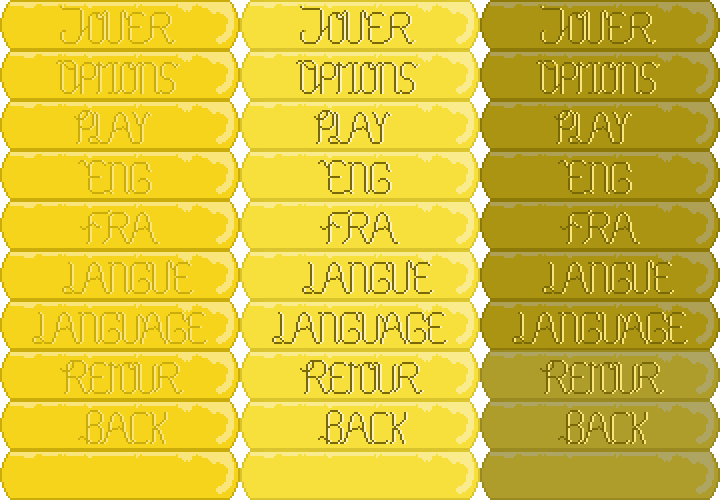
\includegraphics[scale=0.3]{boutons}
\centering
\caption{Spritesheet des boutons utilisés dans le menu}
\end{figure}
\subsubsection{Game}
%toutes les fonctions agissent ici, dans la partie create de phaser.
La state "Game" utilise les fonctions create et update. Dans la fonction create, toutes les actions de jeu sont initiées : le terrain et le personnage sont initiés et les textes du jeu sont traduits.
\begin{lstlisting}[language=JavaScript]
var gameState = {
    create: function(){
        setDialog(gameRef.main.langue);
        createMap1();
        globals.terrainManager.initMap(globals.maps.chateau,true);
        initPlayer(1182,1152)
    },
    update: function(){
        updatePlayer();
        globals.terrainManager.update();
    }
};
\end{lstlisting} 
\textit{Extrait du code de la state "Game".}\\\\
La méthode update est une fonction qui utilise requestAnimationFrame. Sont présentes dans cette fonction, toutes les fonctions qui servent à interagir avec le joueur, c'est à dire la détection de la collision, les changements de maps au contact d'une zone de warp et l'apparition des bulles de dialogues des personnages non-jouables quand le joueur les approche. La fonction qui sert à faire marcher le joueur est aussi présente dans la fonction update.
\subsubsection{Battle}
La state "Battle" est utilisée lors des combats pour initier l'interface de combat. Une nouvelle state est utilisée car il est plus facile de créer un contenu visuel à partir d'une state vide que de modifier une state déjà existante. En effet, la state de combat ne requiert pas une détection de collision ni la création de personnages non-jouables.
\\ Une map de fond est initiée dans la fonction create, ainsi que les personnages à l'écran et leur barres de vie. Le combat est ensuite géré par une classe, battleManager, dont le fonctionnement va être décrit plus loin.
\subsubsection{Transition avec texte}
Cette state sert uniquement à afficher du texte. Une fonction est passée en argument lorsqu'on fait appel à cette state qui l'exécutera. Cette state est une alternative narrative aux cinématiques, trop difficiles à programmer.
\begin{figure}[h]
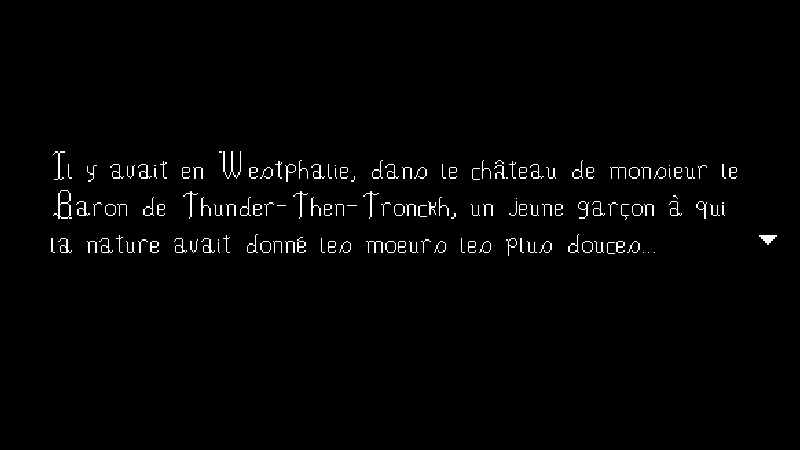
\includegraphics[scale=0.33]{introScreen}
\centering
\end{figure}  
\subsection{Joueur}
%expliquer les déplacements, les directions , les interactions etc...
Le joueur est un sprite qui peut se déplacer lorsqu'une touche directionnelle est enfoncée. Ces déplacements sont activés uniquement quand la propriété "canMove" = true. Cette propriété sert à ce que le personnage ne puisse pas se déplacer pendant les dialogues. Le sprite possède 4 animations de marche qui sont jouées quand l'image se déplace.\\
\begin{figure}[h]
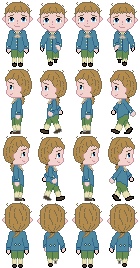
\includegraphics[scale=0.5]{candideSprite}
\centering
\caption{le sprite du joueur avec les différentes frames des animations de marche}
\end{figure}
\\Les déplacements sont détectés dans la fonction updatePlayer appellée dans la state "Game".
\\Ce sprite possède un corps physique (spécificité de Phaser) qui permet les collisions avec son environnement.
\\Le sprite possède également de la vie et des attaques, qui vont être utilisées durant les combats. 
\subsection{Les pnjs}
%expliquer la classe, la bulle (classe) 
%les interaction avec le joueur etc.
\subsubsection{Personnages normaux}
Les pnjs sont une nouvelle classe étendue de la classe sprite de Phaser. Pour créer un nouveau pnj, il faut utiliser :
 \begin{lstlisting}[language=JavaScript]
var myChar = new Pnj(x,y,key,frame,name,dialogs,faceAnimKey);
\end{lstlisting}
Voici l'explication de ces arguments:
\begin{itemize}
\item x,y : Définissent la position du sprite.
\item key : Référence de la spritesheet sous forme de string.
\item frame : Numéro qui définit la frame affichée. ( habituellement 0 pour avoir le personnage de face) 
\item name : Nom du personnage sous forme de string.
\item dialogs : Variable contenant les répliques du personnage.
\item faceAnimKey : Référence à la spritesheet des animations pendant un dialogue sous forme de string.
\end{itemize}
Chaque pnj a une méthode update qui permet de détecter le joueur et créer une interaction avec lui. Le code regarde si le rectangle formé par le sprite du joueur intersecte un autre rectangle plus grand, qui englobe le pnj. Si c'est le cas et que le phylactère du pnj n'est pas encore à l'écran, le personnage crée une bulle. Lorsque la bulle est affichée, le joueur peut appuyer sur "enter" et faire démarrer le dialogue. Cette méthode de détection de bulle a été codée avec des "if" et beaucoup de variables booléennes. Une amélioration serait possible avec des signaux, une spécificité de Phaser, qui permettent l'appel d'une fonction lorsque qu'un événement est déclenché.\subsubsection{Ennemis}
Les ennemis sont une classe étendue de la classe Pnj. Ce sont des pnjs dotés de points de vie et d'attaques pour pouvoir les utiliser lors de combats. Chaque ennemi possède une méthode turn, utilisée lors d'un tour au combat et une méthode startCombat qui fait basculer le jeu sur la state de combat.
\subsection{Les bulles}
Les bulles sont une classe. Chaque bulle est composée de trois parties, le fond, le texte et un triangle animé. Les bulles jouent plusieurs rôles. Elles peuvent indiquer un dialogue mais aussi permettre au joueur de rentrer dans une nouvelle map (grâce à la méthode goToHouse) lorsqu'il y a un élément tel qu'une porte que le joueur doit ouvrir. La détection des zones de warps à bulle est programmée à l'aide de boucles et de "if". Le code pourrait être simplifié à l'aide de signaux Phaser.
\begin{figure}[H]
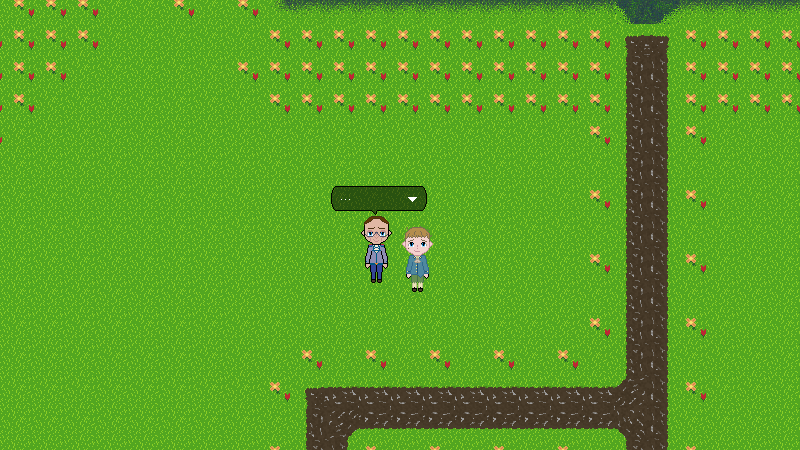
\includegraphics[scale=0.5]{bulleDialog}
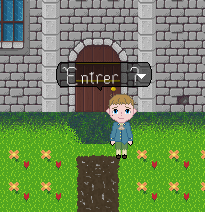
\includegraphics[scale=0.5]{bulleMaison}
\centering
\caption{Exemples de phylactères}
\end{figure}
\subsection{Gestion des dialogues}
%expliquer la police de caractères, la dynamique des choix, l'objet %manager , la syntaxe (les arrays avec les callbacks etc...)
Tout affichage de texte est géré par la classe DialogManager et ses méthodes. 
La méthode start est appelée en premier. Elle affiche une boîte de dialogue et crée un bitmapText vide, un élément graphique de Phaser qui affiche du texte avec une police choisie au préalable. La méthode empêche aussi le joueur de se déplacer. \\
Chaque morceau de texte doit avoir une syntaxe précise pour pouvoir être affiché grâce à la méthode displayText, qui va être décrite plus loin dans le texte. Voici des exemples de syntaxes.
\begin{lstlisting}[language=JavaScript]
	var globals.dialogs.txtSimple = ["texte simple"];
	var globals.dialogs.txtCallback = [
		["texte simple avec callbakc",function(){}]
	];
\end{lstlisting}
\textit{Exemple de la syntaxte d'un texte simple et d'un texte suivi d'une callback}\\
\begin{lstlisting}[language=JavaScript]
	var globals.dialogs.txtChoix = [
		[
			"action avec choix",
			["choix 1","choix 2"],
			[function(){callback 1},function(){callback 2}]
		]
	];
\end{lstlisting} 
\textit{Exemple de syntaxe pour un texte qui comporte des choix}\\
\begin{figure}[h]
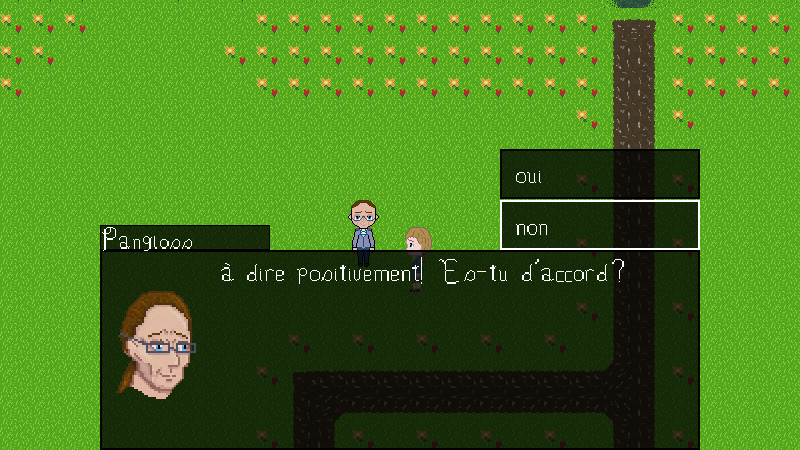
\includegraphics[scale=0.33]{choix}
\centering
\caption{Exemple d'un choix onéreux}

\end{figure}
\subsection{Gestion du terrain}
%expliquer les maps,collisions, tilesets,calques, warps , l'objet terrainmanager etc... expliquer le fail avec le tween manager pour le fade in et fade out.
%expliquer le problème avec les données dans la map et la solution.
\subsection{Gestion des combats}
%expliquer la dynamique de combat, les points de vie etc..
\subsection{Interaction avec les objets}
à compléter idée: un objet possède ou non un callback 

%\subsection{Du code à l'application}
%parler d'éléctron, npm, des packages.json, du favicon, de la fenêtre et des sauvegardes de la partie. (fenêtres)

%\subsection{Publication}
%système de sauvegarde , gitpages
\section{Scénario alternatif}
expliquer les dialogues, conserver le contenu tout en l'adaptant etc...donner des exemples de situations alternatives . et le résultat actuel
expliquer la complication lié au temps, le rabotage etc..
\section{Conception des assets}
\subsection{Visuel}
%logiciels utilisé , techniques(travailler avec des tiles, couches de transparence...)inspiration pour les personnages, dessins originaux etc.. restrictions au niveau du pixel art, base pour cohérence etc...
\subsubsection{Police personnalisée}
%comment on a fait
\subsubsection{Sprites de dialogues}
techniques(couches, dessins - restrictions), exemple 
\subsubsection{Sprites d'overworld}
techniques, exemples
\subsubsection{Tilesets}
techniques, exemples
\subsubsection{Tilemap}
\subsection{Musical}
logiciel utilisé , techniques (trouver une suite d'accord, les instruments etc..) , éventuellement les bruitages , la campanella midi file
\section{Conclusion}
%long !!! --> désillusion XD 
%code à simplifier : signaux
% ce que ça a apporté
% ouverture : continuation du projet
\end{document}
